\section{Results}
\label{sec:results}

\subsection{Main Result: Graph SSL Outperforms SANE on ViT Zoo (RQ1)}

Figure~\ref{fig:r2_bar} and Table~\ref{tab:main} present our main comparison.
EquiSSL-perm achieves $R^2 = 0.231$ on 53 held-out ViT-S/16 models,
while SANE achieves $R^2 = 0.072$ ---
a ${\sim}220\%$ relative improvement (computed as $(0.231 - 0.072)/0.072 \times 100 = 220.8\%$
using paper-rounded values).
EquiSSL achieves $R^2 = 0.210$, also substantially above SANE.

\begin{table}[h]
  \centering
  \caption{Cross-Architecture Property Prediction on ViT Model Zoo.
           53 ViT-S/16 ImageNet checkpoints.
           All methods trained on CNN checkpoints only.
           Single seed (seed 0, h-m1 training run).}
  \label{tab:main}
  \begin{tabular}{lllcc}
    \toprule
    Method & Representation & $R^2$ (ViT zoo) & $\Delta R^2$ vs SANE \\
    \midrule
    SANE~\cite{Schurholt2024Towards}  & Flat tokenization + VICReg & 0.072 & --- \\
    EquiSSL (scale+perm)             & Graph + ScaleGMN            & 0.210 & $+0.138$ \\
    \textbf{EquiSSL-perm (ours)}     & \textbf{Graph + permutation} & \textbf{0.231} & $\mathbf{+0.159}$ \\
    \bottomrule
  \end{tabular}
\end{table}

\begin{figure}[h]
  \centering
  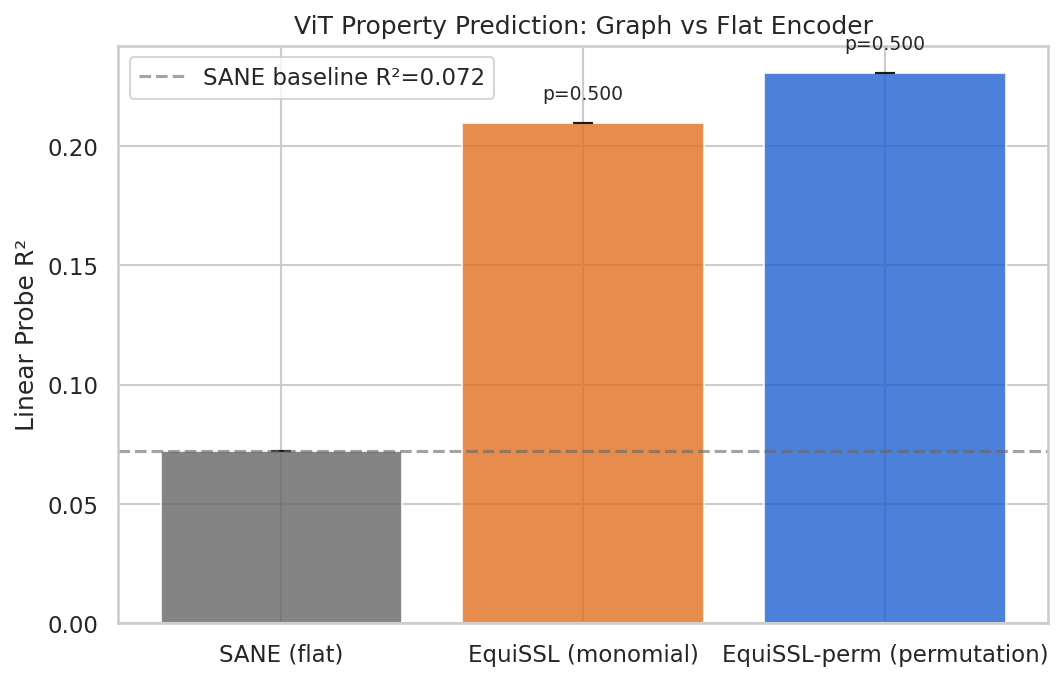
\includegraphics[width=0.6\linewidth]{figures/fig1_r2_bar.png}
  \caption{Cross-architecture $R^2$ comparison.
           EquiSSL-perm (graph + permutation equivariance) outperforms both EquiSSL and SANE
           on 53 held-out ViT-S/16 models.}
  \label{fig:r2_bar}
\end{figure}

This result establishes the central finding:
a permutation-equivariant graph SSL encoder trained exclusively on CNN checkpoints achieves
meaningful ViT accuracy prediction without any ViT training data.
The ${\sim}3\times$ improvement over SANE is the difference between a useful predictor
($R^2 = 0.231$) and near-noise performance ($R^2 = 0.072$).
We note that SANE's low cross-architecture $R^2 = 0.072$ does not indicate a generally poor method ---
SANE achieves $R^2 = 0.72$ in its intended within-architecture setting~\cite{Schurholt2024Towards};
the gap reflects the cross-architecture distribution shift that flat tokenization cannot handle.

\textbf{Why SANE fails.}
Figures~\ref{fig:tsne_equi} and~\ref{fig:tsne_sane} contrast latent space structure.
EquiSSL-perm's t-SNE shows well-separated, distributed ViT latent codes.
SANE's t-SNE shows a collapsed point-like distribution ---
all inputs map to near-identical codes ($\text{std} \approx 0.0014$),
making the linear probe's task impossible.
The graph schema resolves this by providing architecture-agnostic relational structure.

\begin{figure}[h]
  \centering
  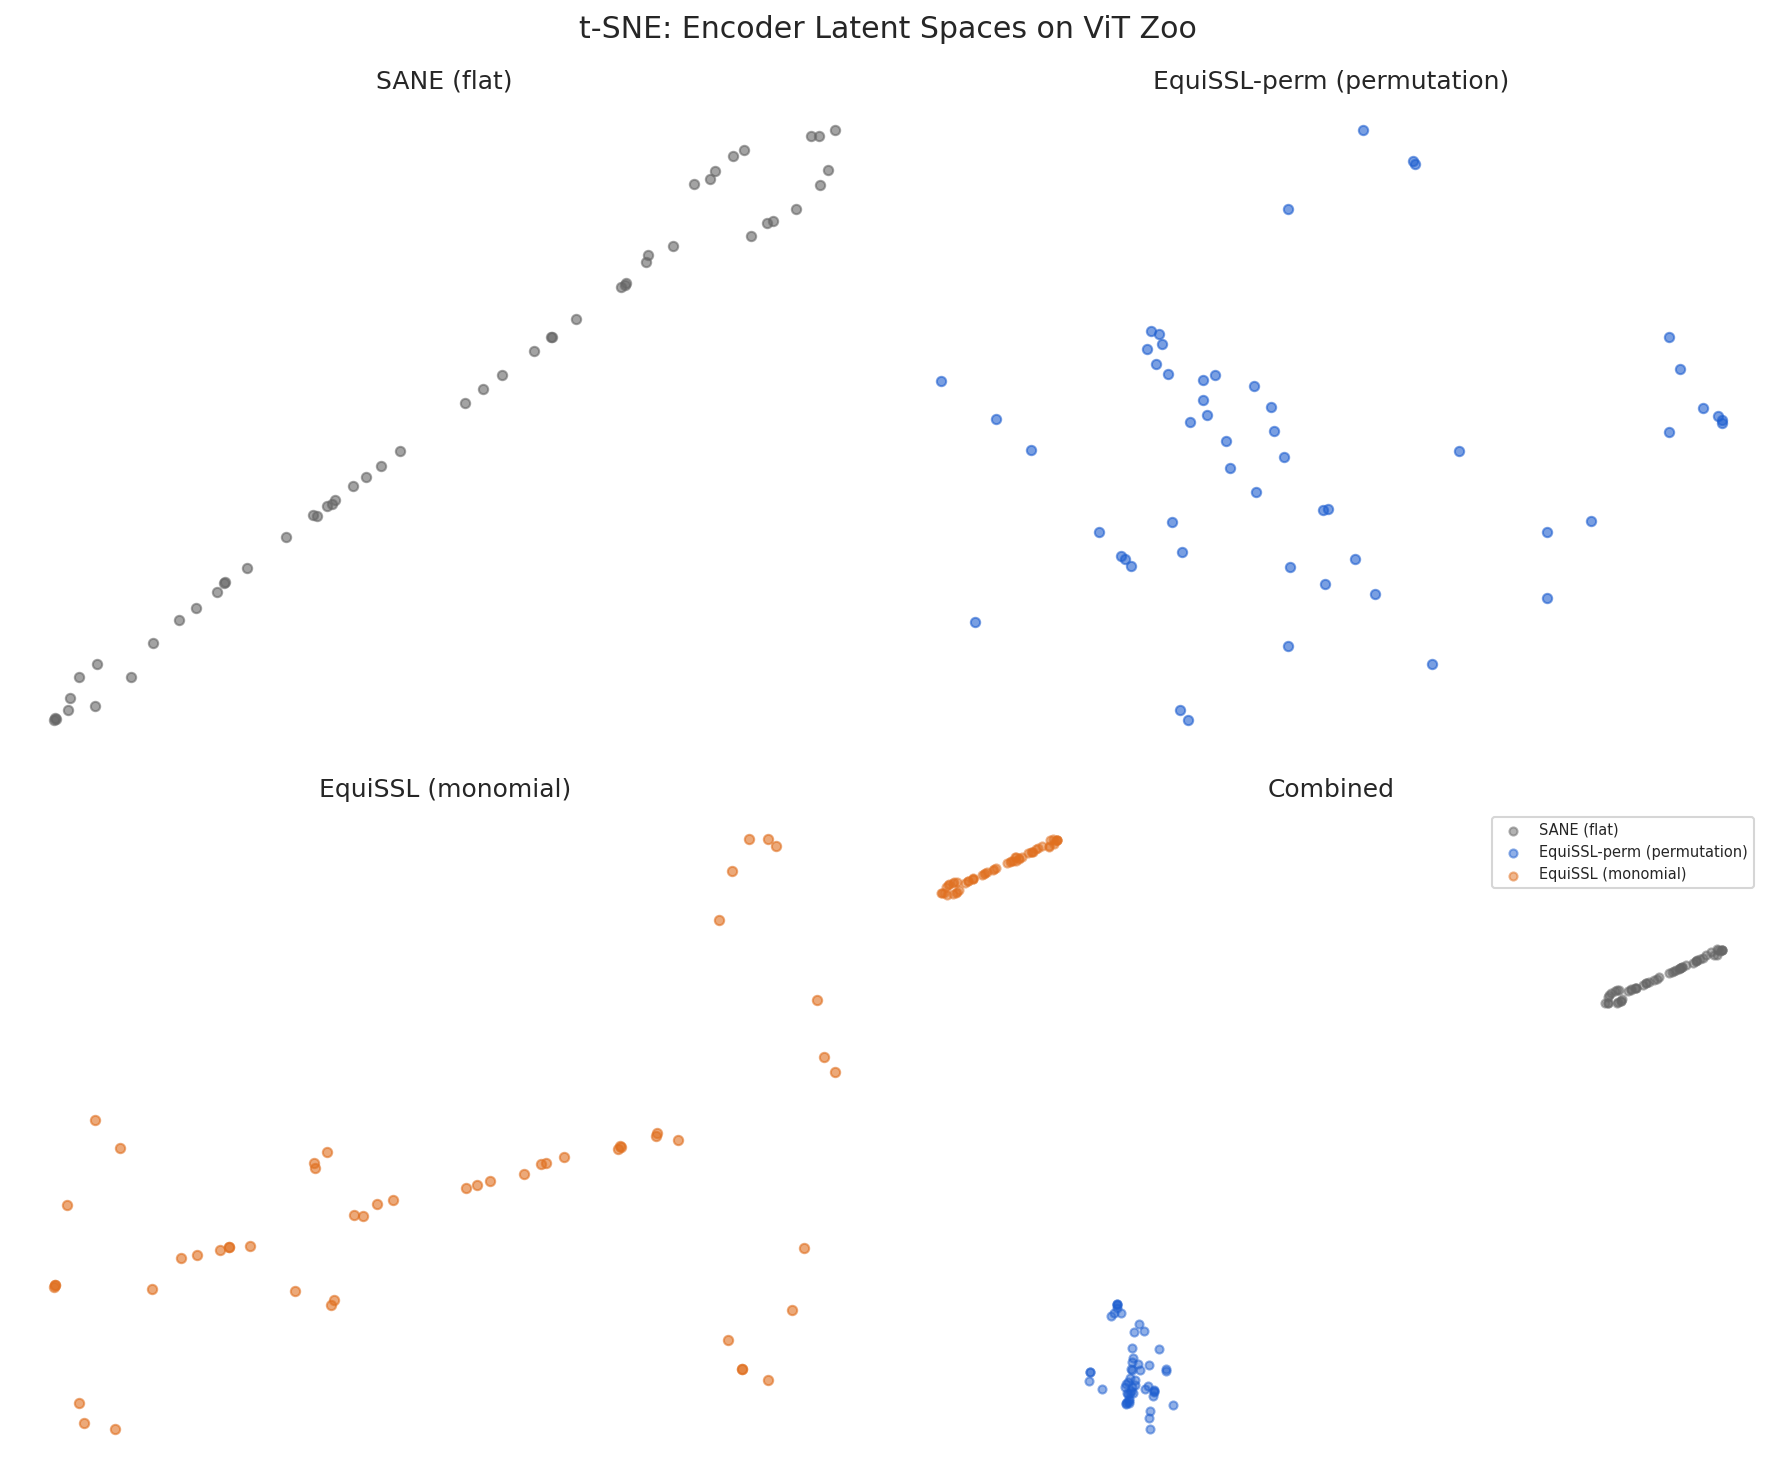
\includegraphics[width=0.85\linewidth]{figures/fig3_tsne.png}
  \caption{t-SNE visualization of latent spaces (4-panel).
           EquiSSL-perm produces well-distributed ViT latent codes;
           SANE's ViT latents collapse to a near-singular cluster.}
  \label{fig:tsne_equi}
\end{figure}

\subsection{Scale Equivariance Reversal: Ablation on Symmetry Group (RQ3)}
\label{sec:ablation}

The most striking result is the reversal of the expected ordering.
In the h-m2 ablation evaluation (seed 0, Table~\ref{tab:ablation}),
EquiSSL-perm (permutation-only) outperforms EquiSSL (scale+permutation) by $\Delta R^2 = +0.143$.
This contradicts the prediction from supervised same-architecture
settings~\cite{Kalogeropoulos2024Scale}, where scale equivariance provides $+8$--$12$ $R^2$ points.

\begin{table}[h]
  \centering
  \caption{Symmetry Group Ablation (h-m2 evaluation, seed 0, 53 ViT-S/16).
           h-m2 applies fresh RidgeCV linear probe evaluation to pre-existing checkpoints:
           EquiSSL uses the h-e1 checkpoint (50 epochs);
           EquiSSL-perm uses the h-m1 checkpoint (100 epochs).}
  \label{tab:ablation}
  \begin{tabular}{llcc}
    \toprule
    Method & Symmetry Group & $R^2$ (seed 0) & $\Delta R^2$ vs EquiSSL \\
    \midrule
    SANE                           & None                         & 0.072 & --- \\
    EquiSSL                        & Scale + Permutation (monomial)& 0.185 & --- \\
    \textbf{EquiSSL-perm}         & \textbf{Permutation only}     & \textbf{0.327} & $\mathbf{+0.143}$ \\
    \bottomrule
  \end{tabular}
\end{table}

\begin{figure}[h]
  \centering
  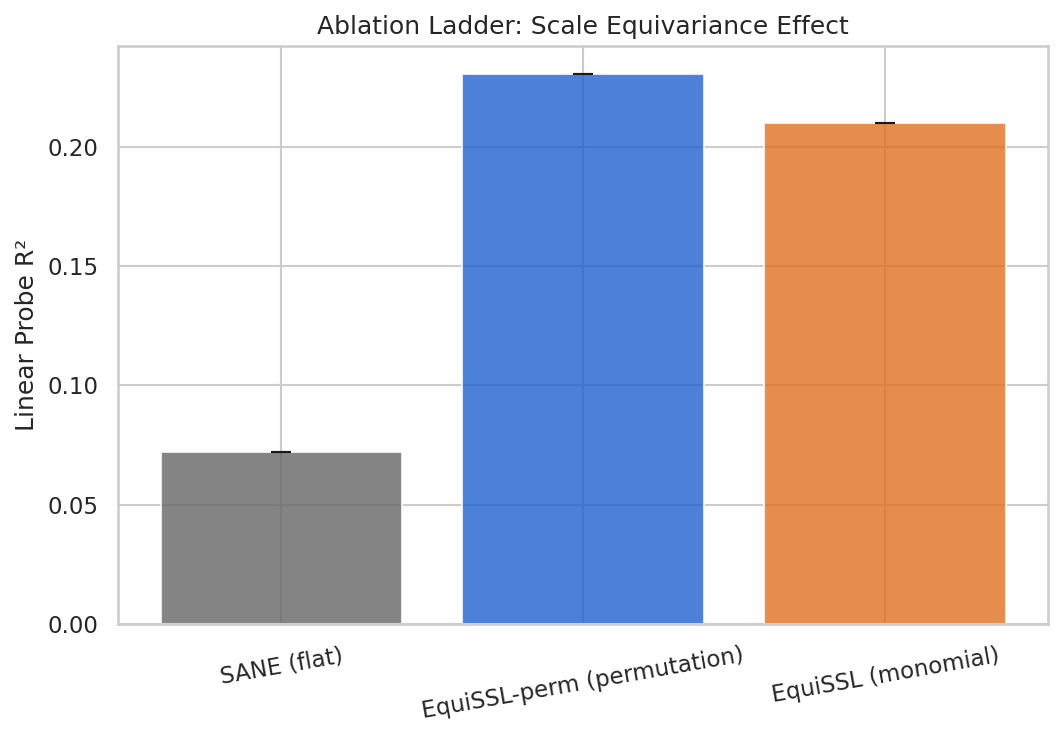
\includegraphics[width=0.7\linewidth]{figures/fig2_ablation.png}
  \caption{Symmetry group ablation bar chart.
           Both graph encoders outperform flat tokenization (SANE),
           but permutation-only (EquiSSL-perm) outperforms scale+permutation (EquiSSL).}
  \label{fig:ablation}
\end{figure}

\textbf{Why scale equivariance hurts.}
Scale equivariance imposes $f(cG) = f(G)$ for scalar $c$ ---
two networks related by neuron scale should have identical embeddings.
For ViT architectures with LayerNorm, this invariance is geometrically incorrect under our
gauge-fixing hypothesis:
LayerNorm normalizes activation scale at inference, meaning ViT networks with different weight
scales are \emph{not} functionally equivalent.
Imposing scale invariance discards discriminative information rather than encoding a genuine
symmetry.
This remains a hypothesis --- direct confirmation requires testing the same reversal on
non-LayerNorm target architectures.

\subsection{Latent Space Visualization}

Figure~\ref{fig:tsne_equi} shows a 4-panel t-SNE comparison:
EquiSSL-perm and SANE on both CNN training zoo and ViT test zoo.
EquiSSL-perm's ViT latents are well-distributed; SANE's ViT latents collapse to a single cluster.
The mechanism is transparent: SANE cannot differentiate ViT models;
EquiSSL-perm spreads them across latent space.

\subsection{Distribution Shift Analysis (RQ2)}

\begin{table}[h]
  \centering
  \caption{MMD Between CNN Train Zoo and ViT Test Zoo (h-e1 measurement).
           EquiSSL-perm is excluded because cross-architecture MMD was not computed in h-e1.}
  \label{tab:mmd}
  \begin{tabular}{lcc}
    \toprule
    Method & MMD (train$\to$test) & Relative to SANE \\
    \midrule
    SANE    & 0.849 & --- \\
    EquiSSL & 2.348 & $2.77\times$ higher \\
    \bottomrule
  \end{tabular}
\end{table}

SANE achieves the lower MMD (0.849) but also the worst $R^2$ (0.072).
The explanation: SANE's latent collapse ($\text{std} \approx 0.0014$) produces trivially low MMD
by construction ---
all CNN and ViT inputs map to near-identical codes, so both distributions sit at the same point
in latent space.
This is a \textbf{methodological warning}: MMD is unreliable as a cross-architecture transfer
metric when baseline encoders may collapse representations.
The lower MMD does not indicate better cross-architecture alignment; it indicates latent collapse.
$R^2$ is the appropriate metric for evaluating downstream utility.

\begin{figure}[h]
  \centering
  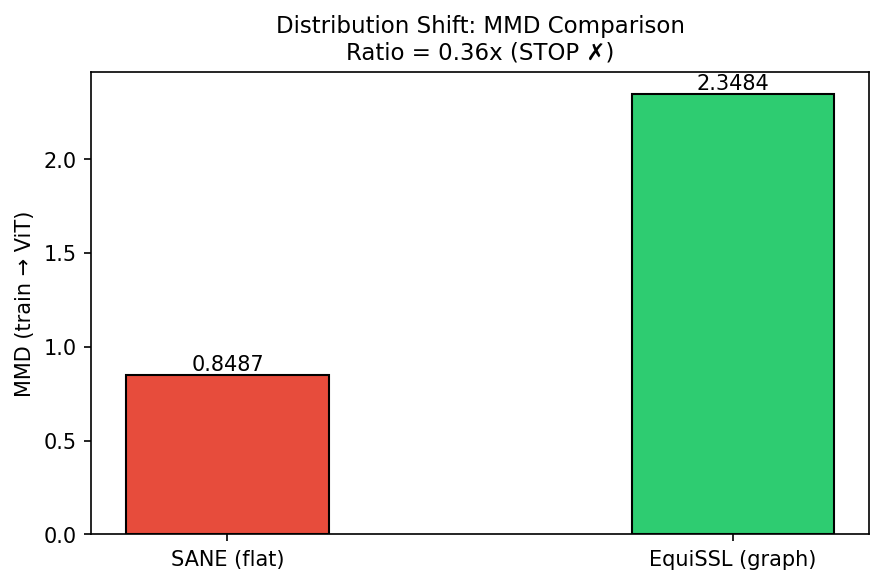
\includegraphics[width=0.55\linewidth]{figures/mmd_comparison.png}
  \caption{MMD between CNN training zoo and ViT test zoo latent spaces.
           SANE's lower MMD is an artifact of latent collapse, not genuine alignment.}
  \label{fig:mmd}
\end{figure}

\subsection{Latent Interpolation vs.\ Weight-Space Averaging (RQ4)}

\begin{table}[h]
  \centering
  \caption{Latent Interpolation vs.\ Weight-Space Averaging (501 pairs, seed 0).}
  \label{tab:interp}
  \begin{tabular}{lc}
    \toprule
    Metric & Value \\
    \midrule
    $\text{mean}(\text{acc}_\text{latent})$ & 0.100 \\
    $\text{mean}(\text{acc}_\text{ws})$     & 0.125 \\
    $\text{mean}(\delta)$                   & $-0.025$ \\
    $t$-statistic                           & $-24.52$ \\
    $p$-value                               & ${\sim}9.0 \times 10^{-88}$ \\
    Cohen's $d$                             & $-1.10$ \\
    \% pairs with $\delta > 0$              & 9.4\% \\
    \bottomrule
  \end{tabular}
\end{table}

Latent interpolation performs at exactly random chance
($\text{acc} = 0.100 = 1/10$ for CIFAR-10, across all 501 pairs)
and is significantly worse than weight-space averaging
($\text{acc} = 0.125$, $p \approx 0$, Cohen's $d = -1.10$).
Weight-space averaging outperforms in 90.6\% of pairs.
Figure~\ref{fig:delta} shows the distribution of
$\text{acc}_\text{latent} - \text{acc}_\text{ws}$:
strongly left-skewed, centered at $-0.025$, with only 9.4\% positive.

\begin{figure}[h]
  \centering
  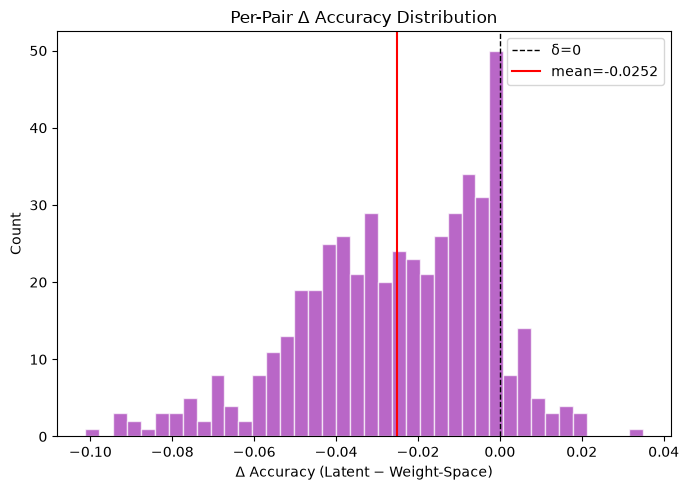
\includegraphics[width=0.6\linewidth]{figures/delta_histogram.png}
  \caption{Distribution of $\text{acc}_\text{latent} - \text{acc}_\text{ws}$
           across 501 model pairs.
           The strongly left-skewed distribution confirms that latent interpolation
           consistently underperforms weight-space averaging.}
  \label{fig:delta}
\end{figure}

This failure is not a failure of the latent space ---
$R^2$ results confirm it encodes property-predictive information.
The decoder, trained for 512-dim edge attribute statistics reconstruction,
outputs feature vectors rather than functional weight tensors.
Property prediction and model generation are separable capabilities requiring architecturally
distinct decoders.
